\section{Datasets}

Several image collections were used for measuring localization performance, both indoors
and outdoors. To ensure continuity and comparability with previous works of~\citet{InLoc,
Bastien}, we utilize the open-source InLoc Dataset presented in the original Inloc
paper~\citep{InLoc}. Another closed-source, indoor dataset is a 3D scanner-generated
digital twin of a SIEMENS manufacturing facility that is targeted by several use cases of
the Industry \& Construction 4.0 Solutions project called ARTwin, financially supported by
the European Union's Horizon 2020 research and innovation program. Finally, an outdoor
dataset is covered by the inclusion of the open-source Phototourism dataset from the Image
Matching Challenge
2021\footnotei{.}{\url{https://www.cs.ubc.ca/research/image-matching-challenge/2021/}}

\subsection{InLoc Dataset}

The dataset consists of a database of Faro 3D scanner-generated RGBD scans that are
geometrically registered to the floor plan of two buildings of Washington University in
St. Louis. The test set is a composition of RGB photos taken by a hand-held device (an
iPhone).

277 RGBD panoramic images have ground truth poses in the global coordinate system spanning
across the floor plan. Each RGBD panoramic scan is a point cloud (\emph{scan}) having
roughly 40~million colored points. The final dataset is generated by obtaining
36~perspective RGBD images from each panorama by extracting standard perspective views
($60^{\circ}$~FoV) with a sampling stride of $30^{\circ}$ in yaw and $\pm30^{\circ}$ in
pitch directions, resulting in cca 10~thousand perspective images in total, examples are
in~\cref{fig:inloc_dataset}. This dataset contains all troublesome elements for indoor
localization, namely repetitive patterns (such as stairs and pillars), global and local
similarities (doors, windows), furniture changing positions in the test set, people moving
across the scene, and textureless, highly symmetric areas (walls, floors, corridors,
classrooms, open spaces).

The original query set consists of 356~photos taken by an iPhone~7 at various lighting
conditions within a day, capturing a variety of occluders and layouts (people, furniture),
also covering only a subset of the floor plan data, with the rest playing the role of
confuser at search time. Ground truth poses for the test set are not publicly accessible,
and evaluation can be done only indirectly via submission to the Visual
Localization\footnote{\url{https://www.visuallocalization.net}} page.

The structure of the dataset's database folder is as follows---\verb|scans/<FLOOR>|
folders, where \verb|FLOOR| is one of DUC1, DUC2, CSE3, CSE4, and CSE5, representing five
floors of the two mentioned buildings (CSE, DUC), contain files named
\verb|<NAME_WITH_SCAN_NUMBER>.ptx.mat| storing RGB and XYZ information of scanned points
in Matlab file format. Every floor has its specific number of scans, uniquely numbered
within a building. Final dataset's perspective views are stored in folders
\verb|cutouts/<FLOOR>/<SCAN_NUMBER>| containing JPG perspective RGB images of size
$1600\times1200$ pixels and MAT files containing bundled RGB perspective image (RGBcut)
and the respective scan points (XYZcut). Files
\verb|alignments/<FLOOR>/transformations/<NAME_WITH_SCAN_NUMBER>.txt| contain $4\times4$
transformation matrices that convert 3D homogeneous points in original .ptx.mat files to
the global coordinate system of the floor plan.

The dataset's query folder contains one subfolder named \verb|iphone7| with the query set
of photos taken by the iPhone camera. Photos are stored as JPG files of size
$4032\times3024$ or $3024\times4032$ pixels, so both landscape and vertical acquisition
modes were used. As the database is landscape, for InLoc algorithm processing, all images
are made landscape, and the ones where the view was changed by rotation are remembered.
Notably, even though sharing the same aspect ratio with the database after such operation,
which InLoc localization pipeline can handle, resizing to the matching dimensions is also
used to speed up the localization performance.

\begin{figure}
    \centering
    \begin{subfigure}{.5\textwidth}
        \centering
        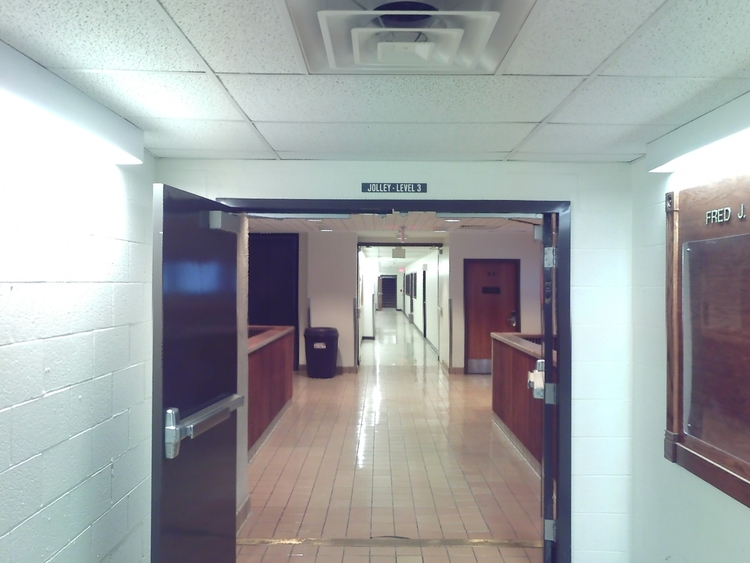
\includegraphics[width=.9\textwidth]{../graphics/cse_cutout_000_90_0.jpg}
    \end{subfigure}%
    \begin{subfigure}{.5\textwidth}
        \centering
        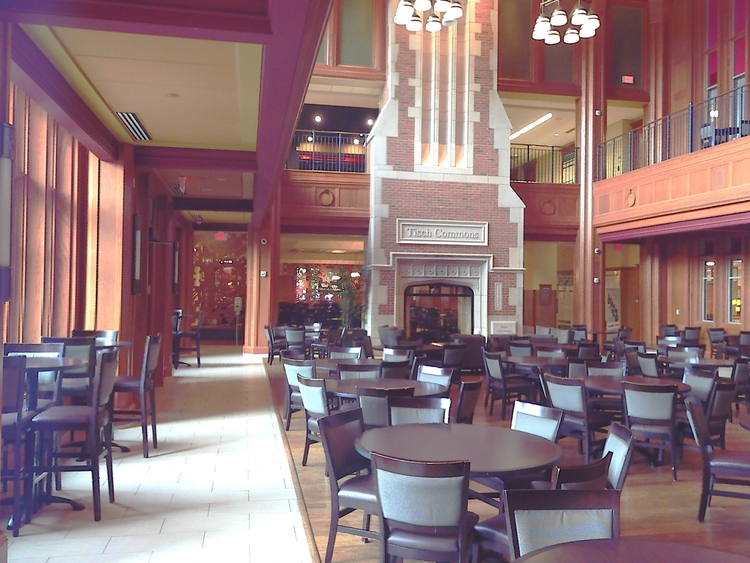
\includegraphics[width=.9\textwidth]{../graphics/DUC_cutout_003_0_0.jpg}
    \end{subfigure}
    \caption{Sample images from InLoc dataset database images.}\label{fig:inloc_dataset}
\end{figure}

\subsection{ARTwin Dataset}

The dataset consists of registered $360^{\circ}$ RGB panoramic images across two halls of
a SIEMENS manufacturing facility together with point clouds for both produced by merging
3D data from a NavVis 3D scanner.

Over the two halls, 29 and 53~panoramic images were obtained. The final dataset used in
this thesis contains roughly 4~thousand processed images and it is generated in accordance
with InLoc Dataset except for a difference in the necessity to remap
$360^{\circ}$~spherical panorama to 2D~surface again, examples are
in~\cref{fig:artwin_dataset}. Hall point clouds are not matched to a common coordinate
system as they overlap when displayed together, so for localization disambiguation one
hall is lifted along the z-axis.

The raw dataset contains all the intermediate files, photos and logs from the acquiring
process together with processed and merged results mentioned above. The structure of the
relevant processed data is \verb|proc/<HALL_ID>|, IDs of the halls are
\verb|2019-09-28_08.31.29| and \verb|2019-09-28_16.11.53|. Within each of these folders,
there is processed point cloud \verb|<HALL_ID>.ply| and \verb|pano| folder with JPG
panoramic scans alongside \verb|pano-poses.csv|. Poses are in the form of 3D scanner
position and orientation quaternion per panoramic scan.

\SaveVerb{hall53}|2019-09-28_16.11.53|
\SaveVerb{hall29}|2019-09-28_08.31.29|
\begin{figure}
	\centering
	\begin{subfigure}{.5\textwidth}
		\centering
		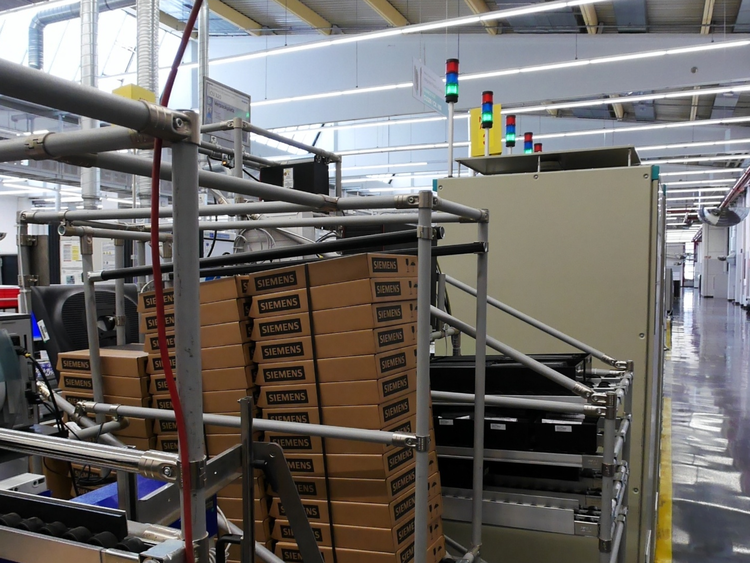
\includegraphics[width=.9\textwidth]{../graphics/2019-09-28_16.11.53_00000_x0_z90_reference.png}
	\end{subfigure}%
	\begin{subfigure}{.5\textwidth}
		\centering
		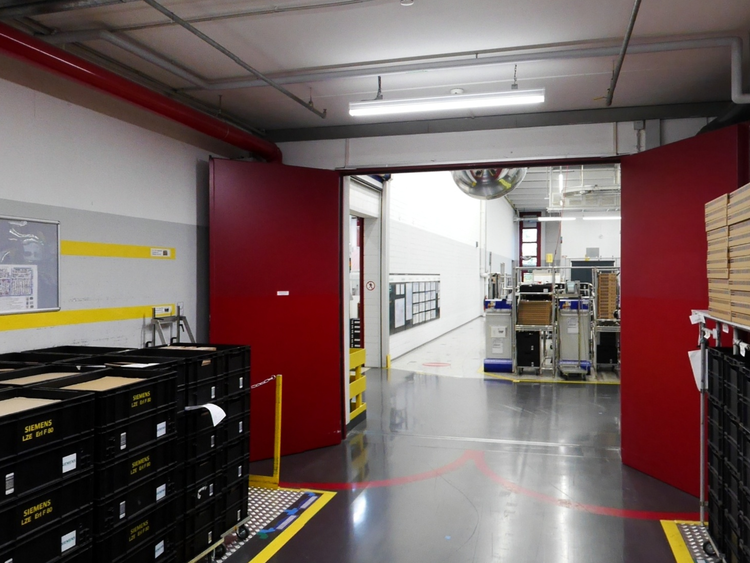
\includegraphics[width=.9\textwidth]{../graphics/2019-09-28_08.31.29_00000_x0_z60_reference.png}
	\end{subfigure}
	\caption{Sample flattened images from ARTwin dataset, on the left hall
        \protect\UseVerb{hall53} is presented, on the right
        \protect\UseVerb{hall29}.}\label{fig:artwin_dataset}
\end{figure}

\subsection{Phototourism Dataset}

The smallest datasets taken from the Image Matching Challenge data, photo-tourism image
collections depicts several popular landmarks, collected from the Yahoo Flickr Creative
Commons 100M (YFCC) dataset. Namely, Hagia Sophia Interior, Pantheon Exterior, and Grand
Place Brussels collections were used. These datasets have around $1\,000$~photos each
coming, using the terminology from~\citet{NRIW}, \uv{from the wild} as they were taken by
many authors, at various distances and with sensor sizes varying considerably, please
see~\cref{fig:imc_dataset}.

\begin{figure}
	\centering
	\begin{subfigure}{.5\textwidth}
		\centering
		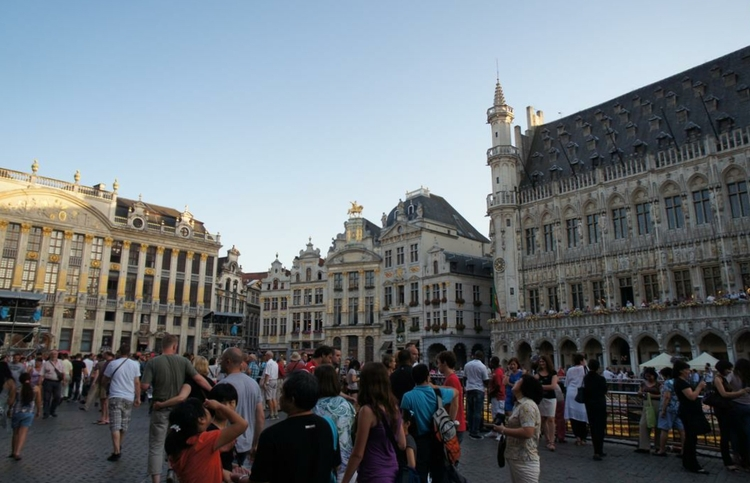
\includegraphics[width=.9\textwidth]{../graphics/grand_06498281_8296173847.jpg}
	\end{subfigure}%
	\begin{subfigure}{.5\textwidth}
		\centering
		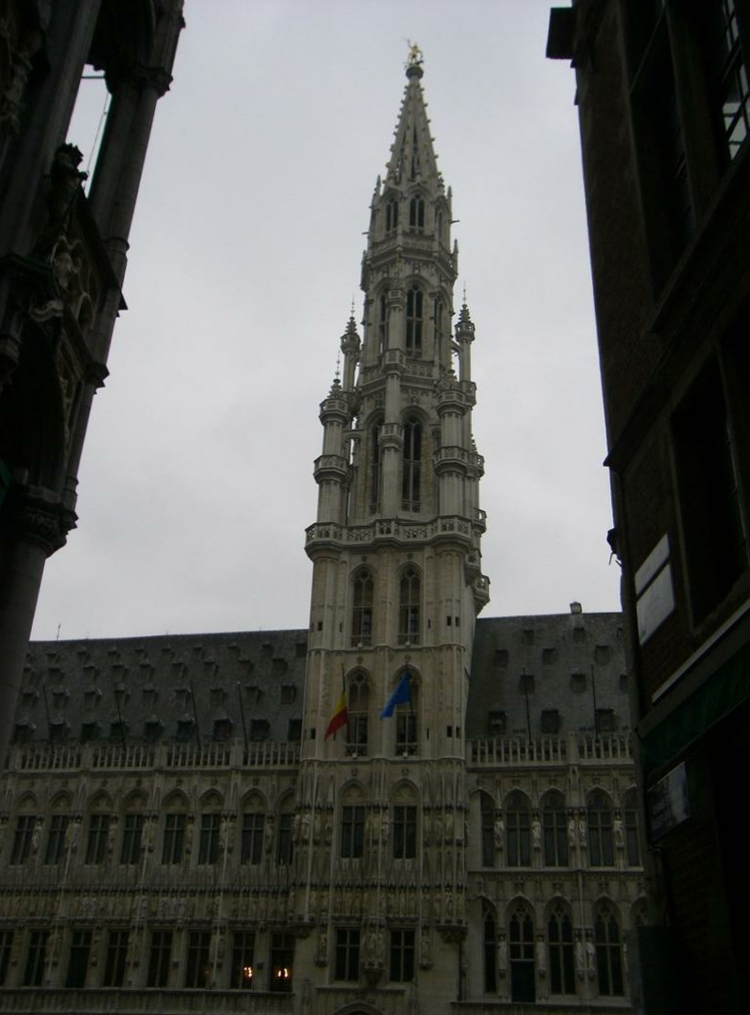
\includegraphics[width=.9\textwidth]{../graphics/grand_01352021_435013564.jpg}
	\end{subfigure}
	\begin{subfigure}{.5\textwidth}
		\centering
		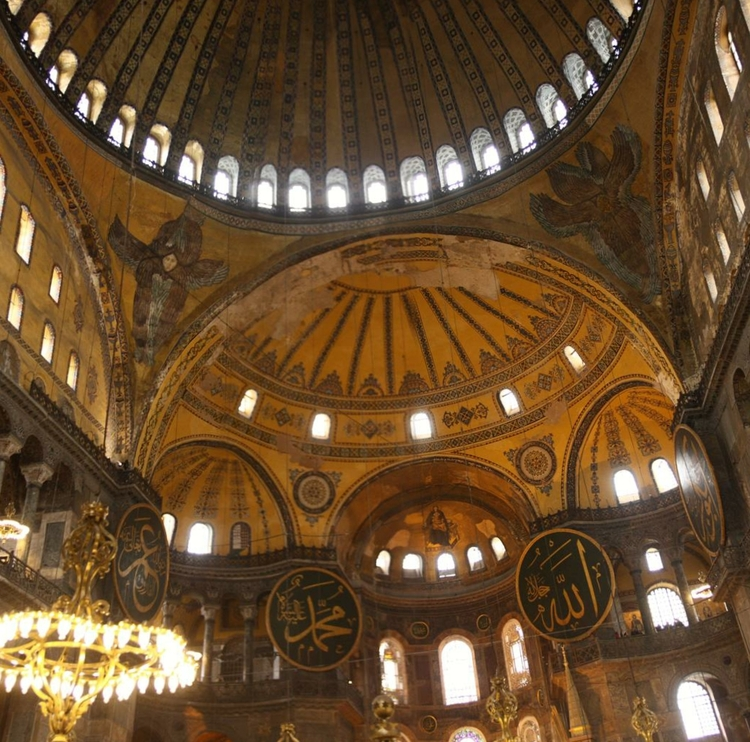
\includegraphics[width=.9\textwidth]{../graphics/hagia_04240457_5644708528.jpg}
	\end{subfigure}%
	\begin{subfigure}{.5\textwidth}
		\centering
		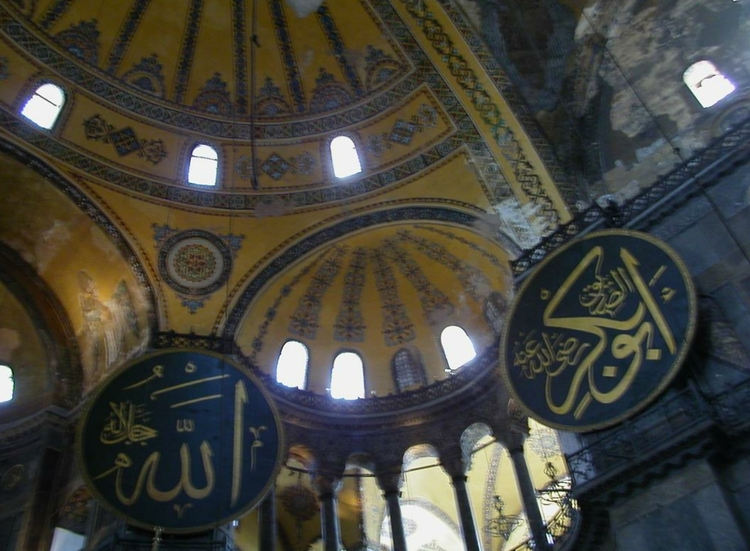
\includegraphics[width=.9\textwidth]{../graphics/hagia_01058134_62294335.jpg}
	\end{subfigure}
	\begin{subfigure}{.5\textwidth}
		\centering
		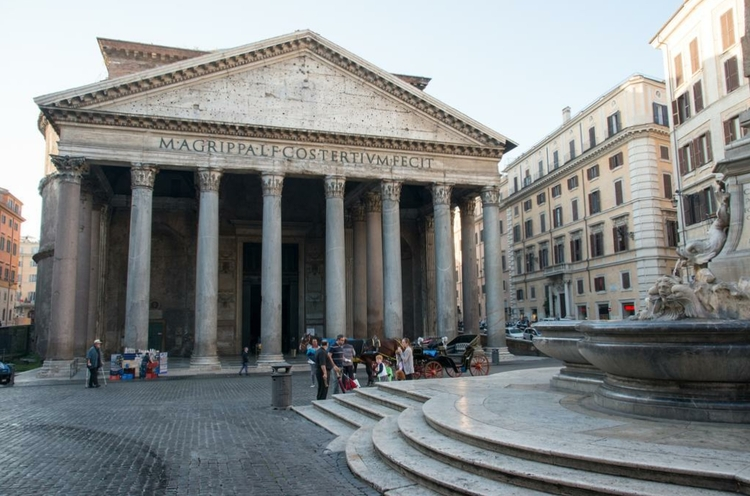
\includegraphics[width=.9\textwidth]{../graphics/pantheon_00488011_10505838106.jpg}
	\end{subfigure}%
	\begin{subfigure}{.5\textwidth}
		\centering
		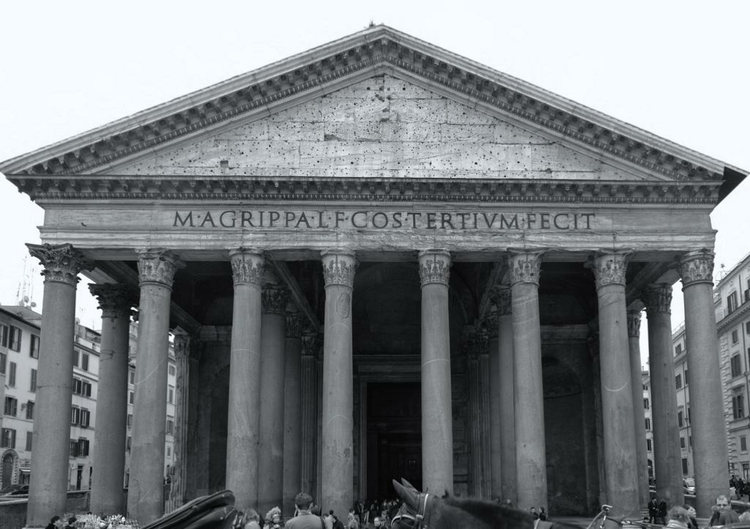
\includegraphics[width=.9\textwidth]{../graphics/pantheon_00927614_8536847775.jpg}
	\end{subfigure}
	\caption{Examples of image collection from Phototourism dataset taken \uv{from
        the wild}, stretching various aspect ratios, sizes, time of the day of the
        aquisition, and varying lighting conditions present in the data. In the top
        row there are images of Grand Place in Brussels, below of interior of Hagia
        Sophia Grand Mosque in Istanbul, and in the bottom of Pantheon in
        Rome.}\label{fig:imc_dataset}
\end{figure}

The dataset per given collection used in the thesis is built on top of raw images by
running COLMAP software. Structure of the COLMAP produced dataset is described in its
documentation\footnotei{.}{\url{https://colmap.github.io/format.html}} Shortly, there is
\verb|dense/sparse/cameras.bin| file with parameters of cameras capturing wild images
retrieved by SfM method implemented in COLMAP, \verb|dense/sparse/images.bin| file with
retrieved 3D positions and orientation quaternions of each image in a common coordinate
system of \verb|dense/fused.ply| point cloud. This point cloud is generated by SfM from
implicit scene representation contrary to the previously mentioned datasets that represent
a 3D scanner-generated approach.\\

Putting everything together---all scene point clouds for all datasets explored in the
thesis are placed in the right-handed coordinate system, though conventions of the
coordinate frames vary, described  side-by-side in~\cref{tab:model_conventions}. In order
to properly render a virtual view, related camera poses must be preprocessed accordingly.
Another side-by-side comparison of the datasets can be found in~\cref{tab:datasets}
presenting their basic statistical features.

\begin{table}
\caption{Comparison of conventions and notations found in scene representations of all
datasets explored in the thesis.}
\centering
    \begin{tabular}{p{4cm} p{4cm} p{4cm}}
    \toprule
    ARTwin & InLoc Dataset & IMC \\
    \midrule
    Right-handed coordinate system, scans use convention where in order to be
    rendered by an OpenGL camera to match database images, in sequence, x-y and y-z axes
    must be switched. There is no notion of global CS where both hall point clouds can be
    placed, so an artificial translation along z-axis is performed on the hall labeled 53
    for localization disambiguation. & Right-handed coordinate system, scans use
    convention where in order to be rendered by an OpenGL camera to match database images,
    in sequence, x-y and y-z axes must be switched. For each scan, a transformation from
    local to the defined global CS is known. & Right-handed coordinate system, model in CV
    notation. To render properly by an OpenGL camera to match database images, y and z
    axes must be inverted.  COLMAP-generated per-view matrices are view matrices.\\
    \bottomrule
    \end{tabular}
\label{tab:model_conventions}
\end{table}

\begin{table}
\caption{Comparison of various features of all datasets used in the thesis.
InLoc test set specified here is generated from the dataset so that we have the ground
truth poses, otherwise the online evaluation tool would need to be used. Number of points
in a scan refers to the mean of points count for iInLoc and ARTwin datasets, and to the
number of points in the whole scene model for the rest. Dimensions are specified in
thousands of pixels and for Phototourism datasets it is not applicable as source photos
have various dimensions.}
\centering
    \begin{tabular}{l c c c c c}
    \toprule
     & InLoc & ARTwin & Hagia Sophia & Pantheon & Grand Place\\
    \midrule
    Train Size  &	7\,977 	& 2\,423    & 670 & 1\,078  & 821\\
    Val Size    &	1\,995	& 379       & 167 & 269     & 205\\
    Test Size   &	356	    & 150       & 50  & 50		& 50\\
    Scan Points	&   40M     & 27M       & 5M  & 5M		& 4M\\
    Dims [k pix]& 1.6x1.2	& 1.6x1.2	& -   & -		& -\\
    \bottomrule
    \end{tabular}
\label{tab:datasets}
\end{table}
